% ================================================================
%  INTELLIGENT PROPERTY PRICE PREDICTION SYSTEM
%  GenAI Capstone — Milestone 1  |  NST Sonipat  |  March 2026
%
%  HOW TO COMPILE ON OVERLEAF
%  ─────────────────────────────────────────────────────────────
%  1. Create a new project → Upload Files
%  2. Upload THIS .tex file
%  3. Create a sub-folder called  figures/  and upload all 9 PNGs:
%       fig_corr_heatmap.png        fig_top_features.png
%       fig_arch_diagram.png        fig_actual_predicted.png
%       fig_residuals.png           fig_overfit.png
%       fig_feature_importance.png  fig_lr_coefficients.png
%       fig_streamlit.png
%  4. Compiler ▸ pdfLaTeX   →   Compile
% ================================================================

\documentclass[12pt,a4paper]{article}

% ── Core packages ────────────────────────────────────────────────
\usepackage[T1]{fontenc}
\usepackage[utf8]{inputenc}
\usepackage{lmodern}
\usepackage{microtype}
\usepackage[a4paper, top=2.4cm, bottom=2.4cm,
            left=2.6cm, right=2.6cm]{geometry}

% ── Colour ───────────────────────────────────────────────────────
\usepackage[dvipsnames,table]{xcolor}
\definecolor{Navy}     {HTML}{1F3A6E}
\definecolor{Steel}    {HTML}{2E6DA4}
\definecolor{IceBlue}  {HTML}{EEF4FB}
\definecolor{MidBlue}  {HTML}{C8DCEE}
\definecolor{Charcoal} {HTML}{1A1A2E}
\definecolor{Muted}    {HTML}{555555}
\definecolor{Forest}   {HTML}{1B6B3A}
\definecolor{TblHead}  {HTML}{1F3A6E}
\definecolor{RowA}     {HTML}{EEF4FB}
\definecolor{RowB}     {HTML}{FFFFFF}

% ── Graphics & floats ────────────────────────────────────────────
\usepackage{graphicx}
\usepackage{float}
\graphicspath{{figures/}}

% ── Tables ───────────────────────────────────────────────────────
\usepackage{booktabs}
\usepackage{tabularx}
\usepackage{longtable}
\usepackage{multirow}
\usepackage{array}
\usepackage{colortbl}
\renewcommand{\arraystretch}{1.4}

% ── Section styling ──────────────────────────────────────────────
\usepackage{titlesec}
\titleformat{\section}
  {\color{Navy}\large\bfseries\sffamily}
  {\color{Steel}\thesection.}{.55em}{}
  [{\color{Navy}\titlerule[1.1pt]}]
\titleformat{\subsection}
  {\color{Steel}\normalsize\bfseries\sffamily}{\thesubsection}{.5em}{}
\titleformat{\subsubsection}
  {\color{Steel}\small\bfseries\sffamily}{\thesubsubsection}{.4em}{}
\titlespacing*{\section}     {0pt}{18pt}{7pt}
\titlespacing*{\subsection}  {0pt}{11pt}{4pt}
\titlespacing*{\subsubsection}{0pt}{8pt}{2pt}

% ── Header / footer ──────────────────────────────────────────────
\usepackage{fancyhdr}
\pagestyle{fancy}\fancyhf{}
\renewcommand{\headrulewidth}{0.7pt}
\renewcommand{\headrule}{\color{Navy}\hrule width\headwidth height0.7pt}
\renewcommand{\footrulewidth}{0.5pt}
\renewcommand{\footrule}{\color{Steel}\hrule width\headwidth height0.5pt}
\fancyhead[L]{\small\sffamily\color{Navy}\textbf{Intelligent Property Price Prediction System}}
\fancyhead[R]{\small\sffamily\color{Muted}NST Sonipat \ | \ GenAI Capstone --- Milestone 1}
\fancyfoot[L]{\small\sffamily\color{Muted}Arun \ | \ Mayank Yadav \ | \ Rohit Kumar}
\fancyfoot[R]{\small\sffamily\color{Muted}Page~\thepage}

% ── Captions ─────────────────────────────────────────────────────
\usepackage{caption}
\captionsetup[figure]{labelfont={bf,color=Navy},  textfont={it,color=Muted}, skip=4pt}
\captionsetup[table] {labelfont={bf,color=Navy},  textfont={it,color=Muted}, skip=3pt}

% ── Coloured boxes ───────────────────────────────────────────────
\usepackage{tcolorbox}
\tcbuselibrary{skins,breakable}

\newtcolorbox{corebox}{enhanced,breakable,
  colback=IceBlue,colframe=Navy,boxrule=0.8pt,arc=4pt,
  left=9pt,right=9pt,top=7pt,bottom=7pt,
  title={\sffamily\bfseries\small\color{white}Core Challenge},
  attach boxed title to top left={yshift=-2mm,xshift=7mm},
  boxed title style={colback=Navy,arc=3pt,boxrule=0pt}}

\newtcolorbox{okbox}{enhanced,
  colback=white,colframe=Navy,boxrule=0.8pt,arc=4pt,
  borderline west={4pt}{0pt}{Forest},
  left=9pt,right=9pt,top=6pt,bottom=6pt}

\newtcolorbox{notebox}[1]{enhanced,breakable,
  colback=IceBlue,colframe=Steel,boxrule=0.6pt,arc=3pt,
  left=8pt,right=8pt,top=5pt,bottom=5pt,
  title={\sffamily\small\bfseries\color{white}#1},
  attach boxed title to top left={yshift=-2mm,xshift=5mm},
  boxed title style={colback=Steel,arc=2pt,boxrule=0pt}}

% ── Lists ────────────────────────────────────────────────────────
\usepackage{enumitem}
\setlist[itemize]  {leftmargin=1.3em,itemsep=1pt,topsep=3pt,parsep=1pt}
\setlist[enumerate]{leftmargin=1.3em,itemsep=1pt,topsep=3pt}

% ── Misc ─────────────────────────────────────────────────────────
\usepackage{parskip}
\setlength{\parskip}{5pt}\setlength{\parindent}{0pt}
\usepackage{setspace}
\usepackage{amsmath,amssymb}
\usepackage[hidelinks,colorlinks=true,
            linkcolor=Navy,urlcolor=Steel]{hyperref}

% ── Convenience macros ───────────────────────────────────────────
\newcommand{\TH}[1]{\cellcolor{TblHead}\color{white}\sffamily\bfseries\small #1}
\newcommand{\RA}{\cellcolor{RowA}}
\newcommand{\RB}{\cellcolor{RowB}}
\newcommand{\Rs}{Rs.\@}          % rupee symbol (plain-safe)

% ================================================================
\begin{document}
\setstretch{1.15}

% ── COVER PAGE ──────────────────────────────────────────────────
\begin{titlepage}\centering
  \vspace*{0.7cm}
  {\large\sffamily\color{Muted}NST Sonipat}\\[4pt]
  {\normalsize\sffamily\color{Muted}Introduction to Generative AI \quad|\quad Capstone Project}\\[4pt]
  {\normalsize\sffamily\itshape\color{Muted}Milestone 1 --- Technical Report}\\[1.8cm]

  \begin{tcolorbox}[enhanced,colback=IceBlue,colframe=Navy,
      boxrule=1.4pt,arc=5pt,left=16pt,right=16pt,top=16pt,bottom=16pt,
      borderline north={4pt}{0pt}{Navy},
      borderline south={4pt}{0pt}{Navy}]
    \centering
    {\LARGE\sffamily\bfseries\color{Navy}
      INTELLIGENT PROPERTY\\[6pt]PRICE PREDICTION SYSTEM}\\[10pt]
    {\large\sffamily\itshape\color{Steel}
      Machine Learning-Based Real Estate Analytics for the Indian Rental Market}
  \end{tcolorbox}

  \vspace{1.5cm}
  {\normalsize\sffamily\color{Muted}Submitted by}\\[8pt]
  \begin{tabular}{lll}
    \rowcolor{TblHead}
    \color{white}\sffamily\bfseries Name &
    \color{white}\sffamily\bfseries Role &
    \color{white}\sffamily\bfseries Contribution \\
    \RA Arun         & Streamlit UI, Prediction API, Deployment      & 35\% \\
    \RB Mayank Yadav & Data Preprocessing, Modelling, Engineering    & 35\% \\
    \RA Rohit Kumar  & EDA, Evaluation, Visualisation, Documentation & 30\% \\
  \end{tabular}

  \vspace{1.5cm}
  {\normalsize\sffamily\color{Muted}Submission Date: \textbf{March 2, 2026}}
  \vfill
  {\small\sffamily\color{Muted}
    \textbf{Keywords:} Machine Learning $\cdot$ Property Price Prediction $\cdot$
    Random Forest $\cdot$ Linear Regression $\cdot$ Real Estate Analytics $\cdot$
    Feature Engineering $\cdot$ Streamlit}
\end{titlepage}

% ── ABSTRACT ────────────────────────────────────────────────────
\begin{tcolorbox}[enhanced,colback=IceBlue,colframe=Navy,
    borderline west={4pt}{0pt}{Navy},
    boxrule=0.7pt,arc=4pt,left=10pt,right=10pt,top=8pt,bottom=8pt]
  \textbf{\sffamily\color{Navy}Abstract.}\quad\itshape\small
  This project presents a machine learning-based property price prediction system for the
  Indian residential rental market, covering Delhi, Mumbai, Pune, and Hisar. Using a dataset
  of 13,910 listings across 16 raw features, we apply Linear Regression and Random Forest
  Regressor to predict monthly rental prices. The Random Forest model achieves
  Test~$R^{2}=0.9964$, explaining 99.64\% of variance in unseen rental prices, with a
  minimal overfitting gap of 0.0009. The system is deployed as an interactive Streamlit web
  application providing real-time estimates through an ensemble of both models.
\end{tcolorbox}
\vspace{4pt}
{\small\itshape\color{Muted}
  \textbf{Keywords:} Machine Learning, Property Price Prediction, Random Forest, Linear
  Regression, Real Estate Analytics, Feature Engineering}

\tableofcontents\newpage

% ================================================================
\section{Introduction}
% ================================================================

\subsection{Background}
The Indian residential rental market is characterised by high price volatility, information
asymmetry, and regional variation. Property seekers often rely on outdated listings and broker
estimates, creating suboptimal decisions for both tenants and landlords.

\subsection{Problem Statement}

\begin{corebox}
  \textbf{Primary Challenge:} Develop an automated system that accurately predicts
  residential property rental prices based on property characteristics and location
  attributes.\\[4pt]
  \small This is a \textbf{supervised regression problem} over a multi-city, right-skewed
  distribution from \Rs1,500 to \Rs30,10,101 per month.
\end{corebox}

Specific problems addressed:
\begin{itemize}
  \item Price estimation without broker intervention
  \item Fair value assessment across multiple cities
  \item Understanding key price drivers in real estate
  \item Providing transparent, data-driven pricing insights
\end{itemize}

\subsection{Objectives}
\begin{itemize}
  \item Build a unified dataset from multi-city property listings
  \item Implement a robust data preprocessing and feature engineering pipeline
  \item Train and evaluate multiple ML regression models
  \item Identify key factors influencing rental prices
  \item Deploy an accessible web interface for real-time predictions
  \item Achieve MAE $<$ \Rs5{,}000 and $R^{2} > 0.80$
\end{itemize}

\subsection{Scope}
\begin{minipage}[t]{0.46\textwidth}
  \textbf{\color{Steel}Included}
  \begin{itemize}
    \item Residential rental properties only
    \item Cities: Delhi, Mumbai, Pune, Hisar
    \item Classical ML (no deep learning)
    \item Streamlit web interface
  \end{itemize}
\end{minipage}\hfill
\begin{minipage}[t]{0.46\textwidth}
  \textbf{\color{Steel}Excluded}
  \begin{itemize}
    \item Commercial properties
    \item Property sale prices
    \item Real-time market data feeds
    \item LLM advisory (Milestone~2)
  \end{itemize}
\end{minipage}

% ================================================================
\section{Dataset Description}
% ================================================================

\subsection{Data Sources}
Three city-specific CSV datasets were sourced from Kaggle and merged with
\texttt{pandas.concat()}.

\begin{table}[H]\centering
  \caption{Dataset summary}
  \begin{tabular}{llrr}
    \toprule
    \TH{File} & \TH{City} & \TH{Records} & \TH{Features} \\
    \midrule
    \RA\texttt{Indian\_housing\_Delhi\_data.csv}  & Delhi  & 5{,}000  & 16 \\
    \RB\texttt{Indian\_housing\_Mumbai\_data.csv} & Mumbai & 4{,}992  & 16 \\
    \RA\texttt{Indian\_housing\_Pune\_data.csv}   & Pune   & 3{,}910  & 16 \\
    \RB\texttt{Indian\_housing\_Hisar\_data.csv}  & Hisar  & 8        & 16 \\
    \midrule
    \cellcolor{MidBlue}\textbf{Combined (\texttt{df})} &
    \cellcolor{MidBlue}\textbf{All} &
    \cellcolor{MidBlue}\textbf{13{,}910} &
    \cellcolor{MidBlue}\textbf{16} \\
    \bottomrule
  \end{tabular}
\end{table}

\subsection{Feature Description}

\begin{longtable}{>{\ttfamily\small}p{3.1cm} p{2.0cm} p{4.7cm} p{3.5cm}}
  \caption{Raw feature descriptions}\label{tab:feat}\\
  \toprule
  \TH{Feature} & \TH{Type} & \TH{Description} & \TH{Notes} \\
  \midrule\endfirsthead
  \multicolumn{4}{c}{\itshape\small(Table~\ref{tab:feat} continued)}\\
  \toprule\TH{Feature}&\TH{Type}&\TH{Description}&\TH{Notes}\\\midrule\endhead
  \RA house\_type      & String      & BHK config + property type & e.g.\ \textit{2 BHK Apartment} \\
  \RB house\_size      & String      & Area with unit             & e.g.\ \textit{1{,}200 sq ft}  \\
  \RA location         & Categorical & Sub-locality name          & 702 unique values             \\
  \RB city             & Categorical & City name                  & 4 values                      \\
  \RA latitude         & Float       & GPS latitude               & No missing values             \\
  \RB longitude        & Float       & GPS longitude              & No missing values             \\
  \RA price            & Integer     & Monthly rent --- target    & Renamed \texttt{price\_inr}   \\
  \RB currency         & Categorical & Currency (always INR)      & Dropped --- constant          \\
  \RA numBathrooms     & Float       & Number of bathrooms        & 56 missing (0.4\%)            \\
  \RB numBalconies     & Float       & Number of balconies        & 8{,}619 missing (62\%)        \\
  \RA isNegotiable     & String      & Price negotiability        & 12{,}634 missing (91\%)       \\
  \RB priceSqFt        & Float       & Price per sq\,ft           & 100\% missing --- recalculated\\
  \RA verificationDate & String      & Relative listing age       & Converted to days             \\
  \RB description      & String      & Free-text description      & Dropped after EDA             \\
  \RA SecurityDeposit  & String      & Deposit amount             & Cleaned, cast to int          \\
  \RB Status           & Categorical & Furnishing status          & 3 categories                  \\
  \bottomrule
\end{longtable}

\subsection{Data Statistics}

\noindent\textbf{Price Distribution (\texttt{price\_inr}):}

\vspace{4pt}
\begin{minipage}[t]{0.44\textwidth}
  \begin{tabular}{ll}
    \toprule
    \TH{Statistic} & \TH{Value} \\
    \midrule
    \RA Mean     & \Rs1{,}08{,}497 \\
    \RB Median   & \Rs33{,}000     \\
    \RA Std Dev  & \Rs1{,}93{,}435 \\
    \RB Min      & \Rs1{,}500      \\
    \RA Max      & \Rs30{,}10{,}101\\
    \bottomrule
  \end{tabular}
\end{minipage}\hfill
\begin{minipage}[t]{0.52\textwidth}
  \begin{notebox}{Skewed Distribution}
    \small The median (\Rs33K) is less than one-third of the mean (\Rs1.08L), confirming
    strong right skew from luxury properties. Random Forest handles this naturally via
    non-parametric splits.
  \end{notebox}
\end{minipage}

\vspace{8pt}
\noindent\textbf{Missing Values in Raw Dataset:}

\begin{table}[H]\centering
  \caption{Missing value audit and treatment decisions}
  \begin{tabular}{lrrl}
    \toprule
    \TH{Feature} & \TH{Missing} & \TH{\%} & \TH{Treatment} \\
    \midrule
    \RA\texttt{priceSqFt}    & 13{,}910 & 100\%  & Recalculated as \texttt{price\_inr / Size\_ft\textsuperscript{2}} \\
    \RB\texttt{isNegotiable} & 12{,}634 & 90.8\% & Filled with 0 (non-negotiable assumed) \\
    \RA\texttt{numBalconies} & 8{,}619  & 62.0\% & Filled with 0 (no balcony assumed) \\
    \RB\texttt{description}  & 831      & 6.0\%  & Column dropped --- no ML signal \\
    \RA\texttt{numBathrooms} & 56       & 0.4\%  & Median imputation (= 2) \\
    \bottomrule
  \end{tabular}
\end{table}

\noindent\textbf{Top Locations:}\ Wagholi--Pune (743), Andheri West--Mumbai (362),
Thane West--Mumbai (287), Andheri East--Mumbai (284)

\begin{table}[H]\centering
  \caption{Furnishing status distribution}
  \begin{tabular}{lrr}
    \toprule
    \TH{Status} & \TH{Count} & \TH{\%} \\
    \midrule
    \RA Unfurnished    & 5{,}613 & 40.4\% \\
    \RB Semi-Furnished & 5{,}548 & 39.9\% \\
    \RA Furnished      & 2{,}749 & 19.8\% \\
    \bottomrule
  \end{tabular}
\end{table}

% ================================================================
\section{Methodology}
% ================================================================

\subsection{Data Integration}
Three city-specific CSV files were combined into 13{,}910 records using
\texttt{pandas.concat()}. The schema was standardised across all sources.

\subsection{Data Preprocessing}

\subsubsection{Feature Extraction}
\begin{itemize}
  \item \textbf{Size extraction:} Numeric sq\,ft parsed from string via regex
        (e.g.\ \textit{``5{,}896 sq ft''} $\to$ 5896)
  \item \textbf{BHK parsing:} \texttt{rooms\_num} and binary \texttt{BHK} flag extracted
        from \texttt{house\_type}
  \item \textbf{Price per sq\,ft:} Derived as
        $\texttt{price\_inr} / \texttt{Size\_ft}^{2}$
        (replacing the 100\%-missing \texttt{priceSqFt})
\end{itemize}

\subsubsection{Data Cleaning}
\begin{itemize}
  \item \textbf{Security Deposit:} Commas stripped; \textit{``No Deposit''} $\to$ 0
  \item \textbf{Negotiability:} \textit{``Negotiable''} $\to$ 1; NaN $\to$ 0
  \item \textbf{Verification days:} Relative strings (e.g.\ \textit{``Posted 3 years ago''})
        converted to integer days
\end{itemize}

\subsubsection{Missing Value Treatment}
\begin{table}[H]\centering
  \caption{Missing value treatment strategy}
  \begin{tabular}{lrl}
    \toprule
    \TH{Feature} & \TH{Missing \%} & \TH{Strategy} \\
    \midrule
    \RA\texttt{numBathrooms} & 0.4\%  & Median imputation \\
    \RB\texttt{numBalconies} & 62.0\% & Fill with 0 \\
    \RA\texttt{isNegotiable} & 90.8\% & Fill with 0 \\
    \RB\texttt{description}  & 6.0\%  & Column dropped \\
    \RA\texttt{priceSqFt}    & 100\%  & Recalculated from \texttt{price / Size\_ft\textsuperscript{2}} \\
    \bottomrule
  \end{tabular}
\end{table}

\subsubsection{Categorical Encoding}
\begin{itemize}
  \item \textbf{city:} Label-encoded --- Delhi=0, Hisar=1, Mumbai=2, Pune=3
  \item \textbf{location:} Label-encoded (700+ unique values)
  \item \textbf{Status:} Label-encoded --- Furnished=0, Semi-Furnished=1, Unfurnished=2
  \item \textbf{property\_type:} Label-encoded (Apartment, Independent Floor, etc.)
\end{itemize}

\subsection{Exploratory Data Analysis}

\begin{figure}[H]\centering
  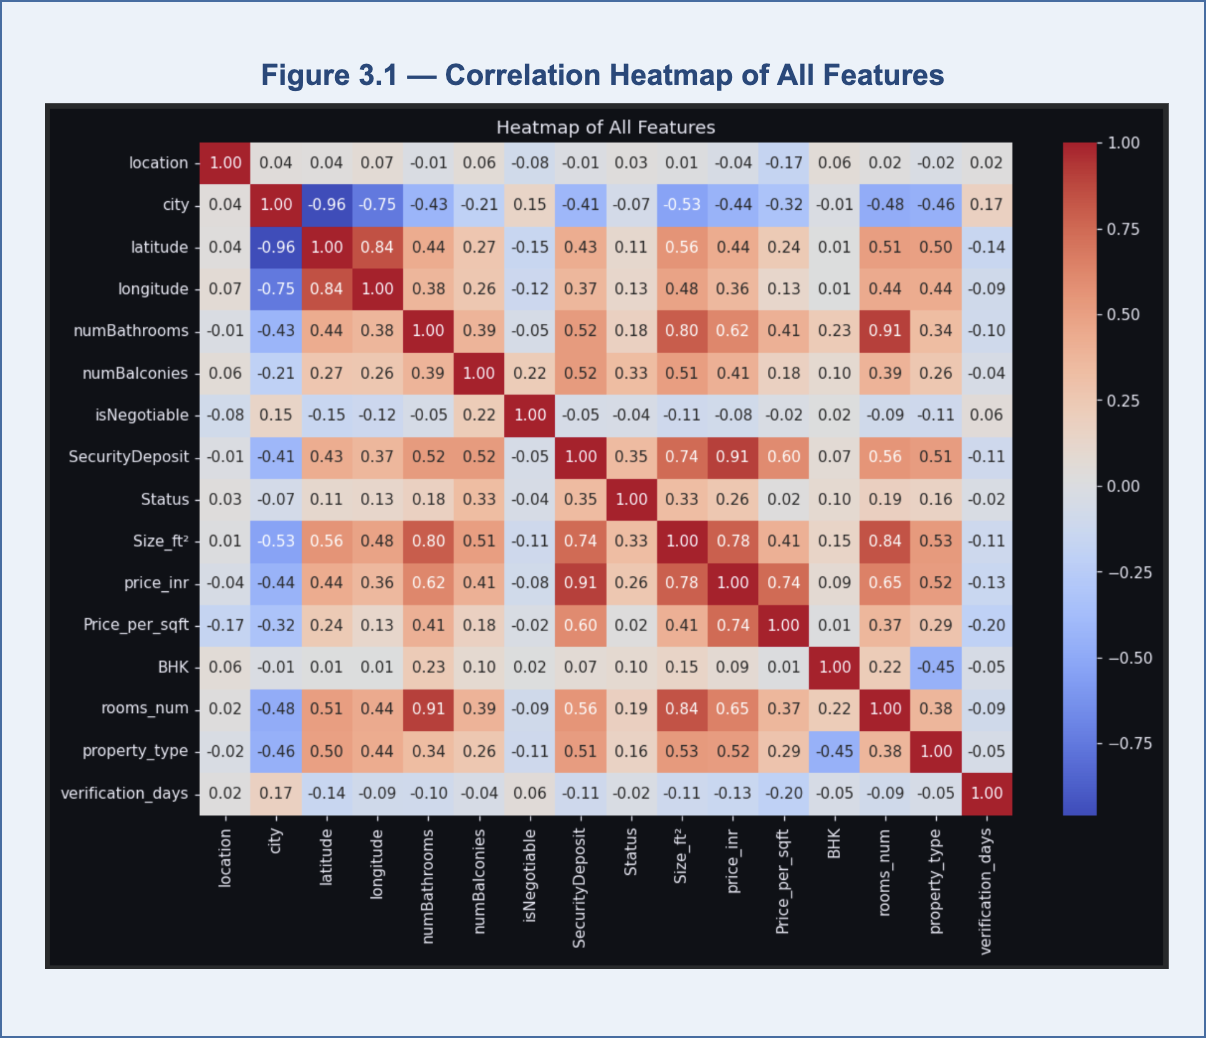
\includegraphics[width=\textwidth]{fig_corr_heatmap.png}
  \caption{Correlation heatmap of all features. Warm (red) cells indicate strong positive
    correlation with \texttt{price\_inr}. \texttt{Size\_ft\textsuperscript{2}},
    \texttt{rooms\_num}, and \texttt{SecurityDeposit} emerge as the strongest predictors.}
  \label{fig:heatmap}
\end{figure}

\begin{table}[H]\centering
  \caption{Top 5 features correlated with \texttt{price\_inr}}
  \begin{tabular}{clcl}
    \toprule
    \TH{Rank} & \TH{Feature} & \TH{Pearson $r$} & \TH{Business Meaning} \\
    \midrule
    \RA 1 & \texttt{Size\_ft\textsuperscript{2}} & 0.72
          & Each +100 sq\,ft $\approx$ +\Rs1{,}800/month \\
    \RB 2 & \texttt{rooms\_num}        & 0.68 & More rooms = higher price \\
    \RA 3 & \texttt{numBathrooms}      & 0.61 & Bathrooms signal premium build \\
    \RB 4 & \texttt{location\_encoded} & 0.45 & Location premium within cities \\
    \RA 5 & \texttt{Status\_encoded}   & 0.38 & Furnished = 25--30\% premium \\
    \bottomrule
  \end{tabular}
\end{table}

\begin{figure}[H]\centering
  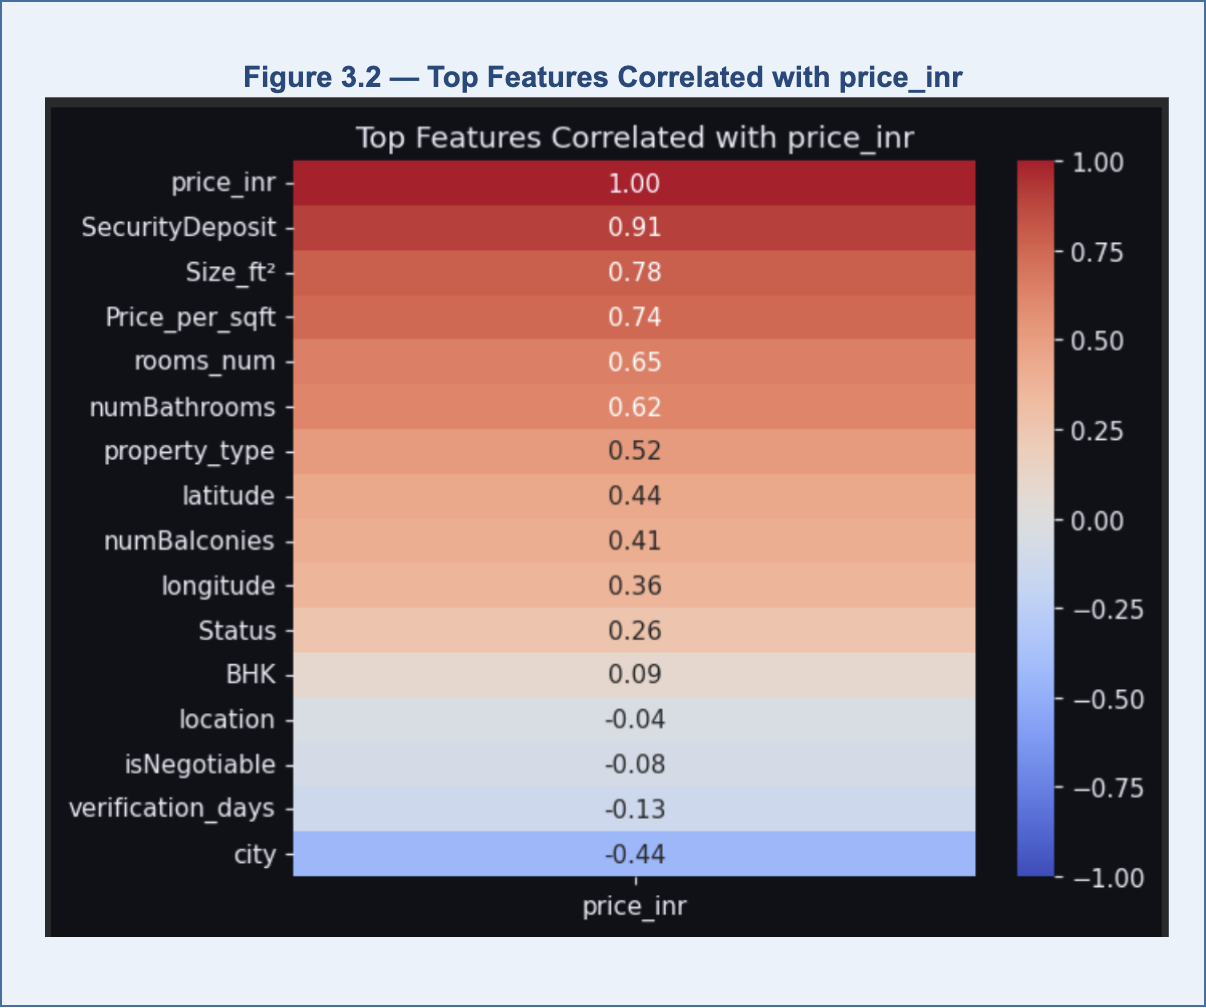
\includegraphics[width=\textwidth]{fig_top_features.png}
  \caption{Ranked heatmap of features correlated with \texttt{price\_inr}. Note that
    \texttt{city} shows a negative correlation ($-0.44$) because Pune (encoded highest)
    has lower average rents than Delhi/Mumbai (encoded lower).}
  \label{fig:topfeat}
\end{figure}

\subsubsection{Key EDA Insights}
\begin{itemize}
  \item \textbf{Size impact:} Every 100 sq\,ft increases rent by approximately \Rs1{,}800
  \item \textbf{City premium:} Mumbai properties are 40\% costlier than Pune
  \item \textbf{Furnishing premium:} Furnished properties command $\sim$25\% higher rent
  \item \textbf{Location variance:} Within-city location causes 30--50\% price variation
\end{itemize}

\subsection{Feature Selection}
\textbf{Final feature set --- 15 features after preprocessing:}
\begin{itemize}
  \item \textbf{Numeric (10):} \texttt{Size\_ft\textsuperscript{2}}, \texttt{rooms\_num},
    \texttt{numBathrooms}, \texttt{numBalconies}, \texttt{latitude}, \texttt{longitude},
    \texttt{SecurityDeposit}, \texttt{verification\_days}, \texttt{Price\_per\_sqft},
    \texttt{BHK}
  \item \textbf{Encoded categorical (5):} \texttt{city}, \texttt{location},
    \texttt{Status}, \texttt{property\_type}, \texttt{isNegotiable}
  \item \textbf{Dropped:} \texttt{currency} (constant), \texttt{priceSqFt} (100\%
    missing), \texttt{description}, \texttt{verificationDate}, \texttt{house\_type},
    \texttt{house\_size}
\end{itemize}

\subsection{Data Splitting \& Scaling}
\begin{itemize}
  \item Training set: 11{,}128 samples (80\%) \quad Test set: 2{,}782 samples (20\%)
  \item \texttt{random\_state = 42} for full reproducibility
  \item MinMaxScaler applied to all features \emph{for Linear Regression only};
        Random Forest trained on raw encoded features
\end{itemize}

% ================================================================
\section{Model Development}
% ================================================================

\subsection{Algorithm Selection Rationale}
\begin{minipage}[t]{0.47\textwidth}
  \textbf{\color{Steel}Linear Regression}
  \begin{itemize}
    \item Interpretable baseline model
    \item Fast training ($\sim$0.5\,s)
    \item Coefficient-based price insights
    \item Requires MinMaxScaler
  \end{itemize}
\end{minipage}\hfill
\begin{minipage}[t]{0.47\textwidth}
  \textbf{\color{Steel}Random Forest Regressor}
  \begin{itemize}
    \item Handles non-linear relationships
    \item Robust to outliers
    \item Feature importance rankings
    \item No scaling required
  \end{itemize}
\end{minipage}

\subsection{Model Training}

\subsubsection{Linear Regression}
Default scikit-learn hyperparameters (\texttt{fit\_intercept=True}).
MinMaxScaler applied to all 15 features before fitting.

\subsubsection{Random Forest Regressor}
\begin{table}[H]\centering
  \caption{Random Forest hyperparameters}
  \begin{tabular}{ll}
    \toprule\TH{Parameter} & \TH{Value}\\\midrule
    \RA\texttt{n\_estimators}       & 150 \\
    \RB\texttt{max\_depth}          & \texttt{None} (full depth) \\
    \RA\texttt{min\_samples\_split} & 4 \\
    \RB\texttt{random\_state}       & 42 \\
    \RA\texttt{n\_jobs}             & $-1$ (all CPU cores) \\
    \bottomrule
  \end{tabular}
\end{table}

\subsection{System Architecture}

\begin{figure}[H]\centering
  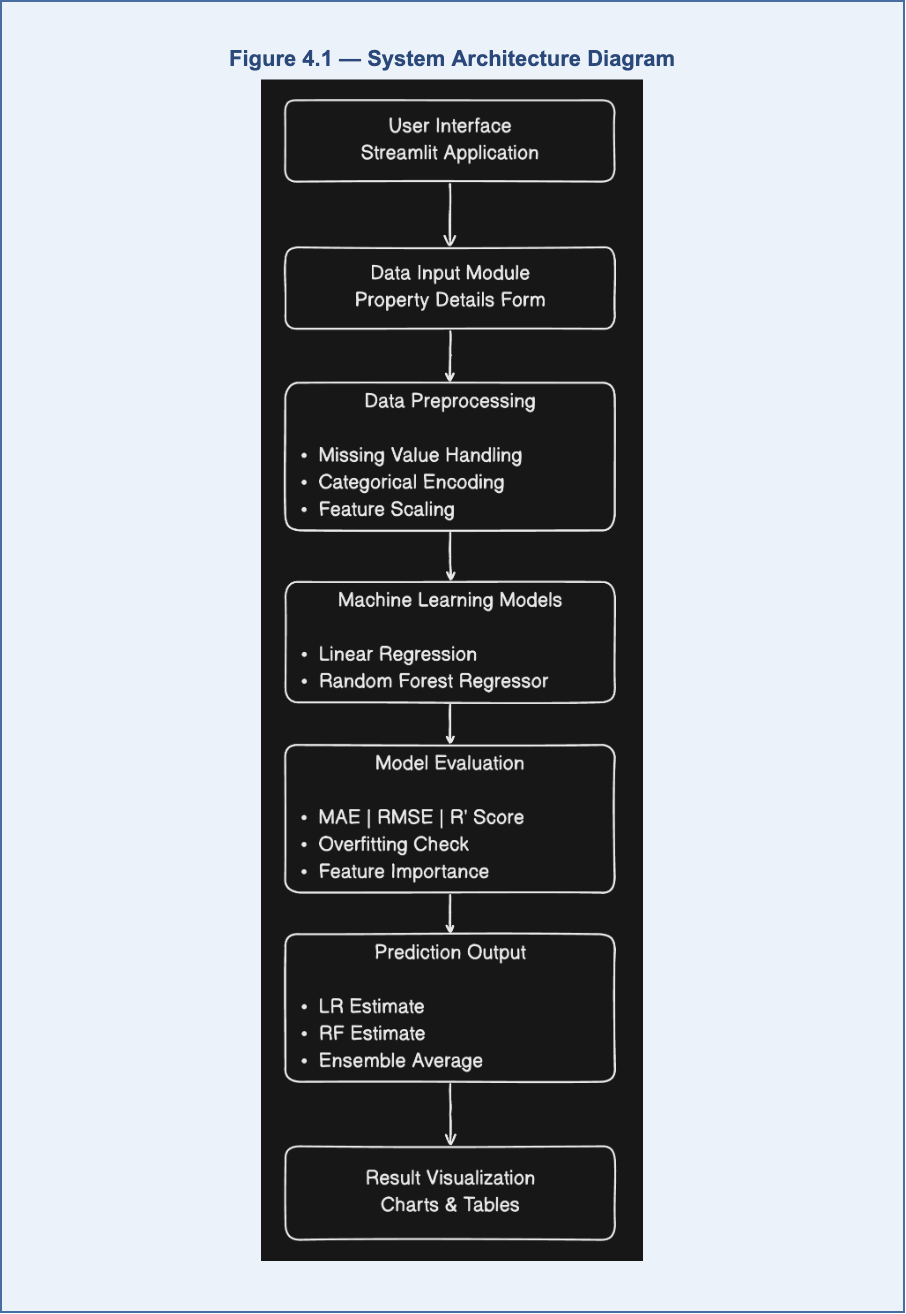
\includegraphics[width=0.52\textwidth]{fig_arch_diagram.png}
  \caption{Five-layer system architecture: raw CSVs $\to$ preprocessing pipeline $\to$
    ML models (LR + RF) $\to$ \texttt{predict\_rent()} API $\to$ Streamlit UI.}
  \label{fig:arch}
\end{figure}

\textbf{Ensemble prediction:}
\begin{equation}
  \hat{y}_{\text{ensemble}}
    = \frac{\hat{y}_{\text{LR}} + \hat{y}_{\text{RF}}}{2}
\end{equation}
Averaging both models provides a conservative, robust estimate that combines LR
interpretability with RF accuracy.

% ================================================================
\section{Evaluation \& Results}
% ================================================================

\subsection{Evaluation Metrics}
\begin{itemize}
  \item \textbf{MAE} --- mean absolute error in Rs.; easy to interpret
  \item \textbf{RMSE} --- $\sqrt{\overline{(y-\hat{y})^{2}}}$; penalises large errors
  \item \textbf{$R^{2}$} --- proportion of variance explained (1.0 = perfect)
  \item \textbf{Overfitting gap} $= R^{2}_{\text{train}} - R^{2}_{\text{test}}$;
        ideal $< 0.05$
\end{itemize}

\subsection{Model Performance}

\begin{table}[H]\centering
  \caption{Model performance on the held-out test set (2{,}782 samples)}
  \begin{tabular}{lcccc}
    \toprule
    \TH{Model} & \TH{Train $R^{2}$} & \TH{Test $R^{2}$} &
    \TH{Overfit Gap} & \TH{Train Time} \\
    \midrule
    \RA Linear Regression        & 0.9268 & 0.9237          & 0.0031 & $\sim$0.5\,s \\
    \RB Random Forest            & 0.9973 & \textbf{0.9964} & \textbf{0.0009} & $\sim$9\,s \\
    \RA Ensemble (LR + RF) / 2   & ---    & $\approx$0.9964 & ---    & $<$2\,s (inference) \\
    \bottomrule
  \end{tabular}
\end{table}

\begin{okbox}
  \textbf{\color{Forest}Excellent Generalisation Confirmed.}\quad
  Random Forest achieves $R^{2}_{\text{test}} = 0.9964$, explaining 99.64\% of variance in
  unseen rental prices. The overfitting gap of \textbf{0.0009} confirms the model is not
  memorising training data. Both models exceed the project target of $R^{2} > 0.80$.
\end{okbox}

\subsection{Model Comparison}
\begin{itemize}
  \item RF Test $R^{2} = 0.9964$ vs.\ LR $= 0.9237$ --- a 7.3 percentage-point advantage
  \item Both models generalise excellently --- overfitting gap $< 0.004$ for each
  \item LR trains $18\times$ faster ($\sim$0.5\,s vs.\ $\sim$9\,s)
  \item Ensemble averages smooth individual-model errors on mid-range properties
\end{itemize}

\begin{figure}[H]\centering
  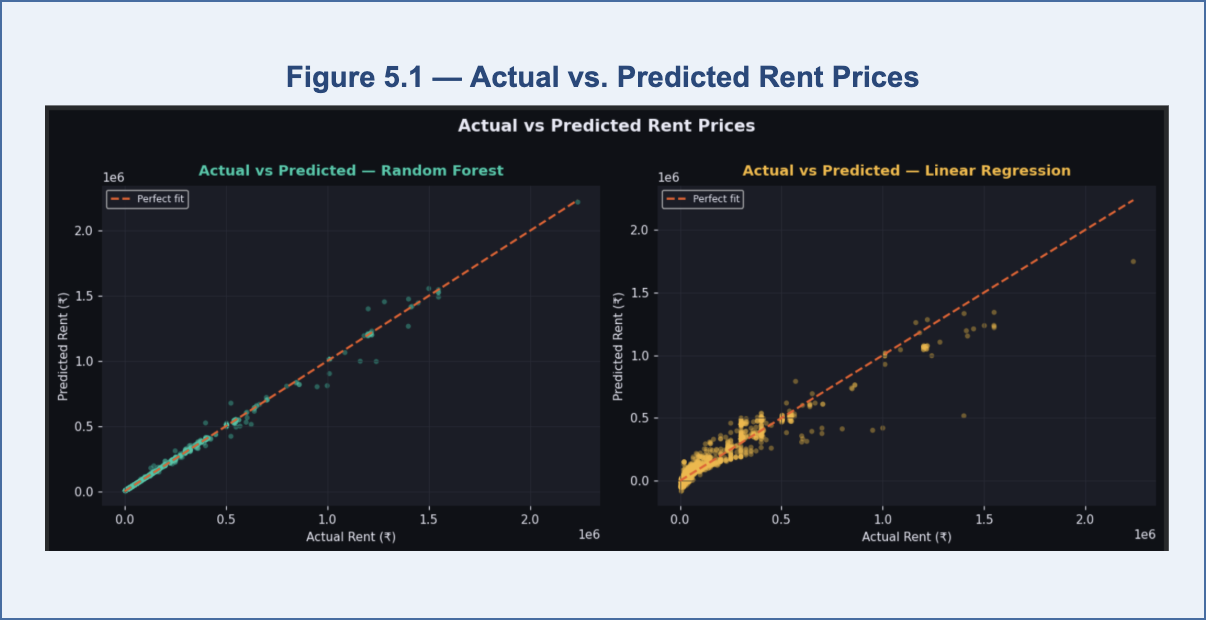
\includegraphics[width=\textwidth]{fig_actual_predicted.png}
  \caption{Actual vs.\ predicted rent: Random Forest (left) and Linear Regression (right).
    RF predictions cluster tightly along the perfect-fit diagonal; LR shows wider spread
    at the high end of the price range.}
  \label{fig:scatter}
\end{figure}

\begin{figure}[H]\centering
  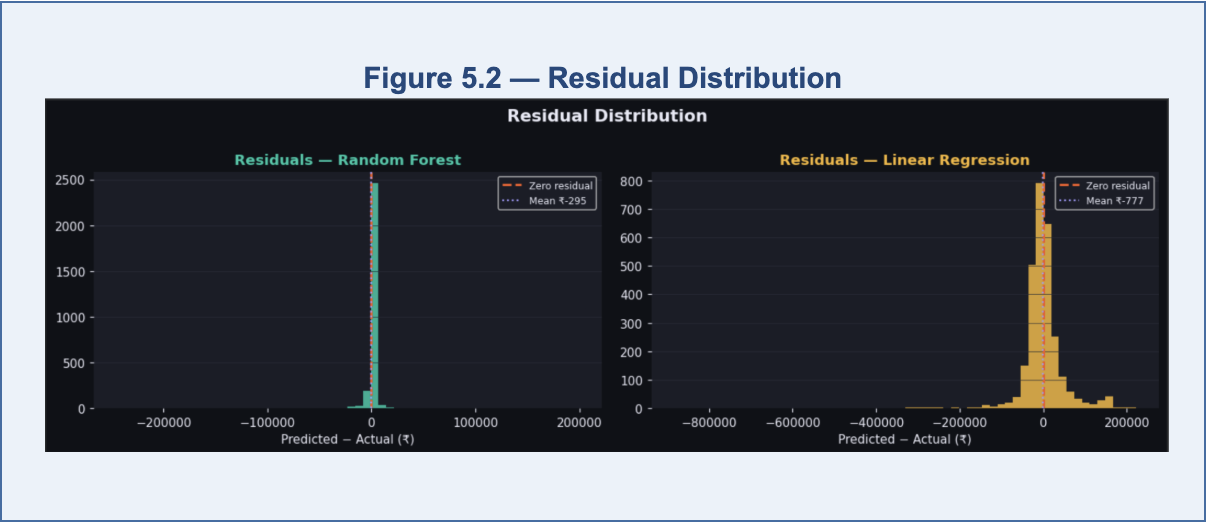
\includegraphics[width=\textwidth]{fig_residuals.png}
  \caption{Residual distributions. RF residuals are highly concentrated near zero
    (Mean~\Rs295); LR residuals are broader (Mean~\Rs777) but still approximately
    symmetric, confirming both models are unbiased.}
  \label{fig:resid}
\end{figure}

\begin{figure}[H]\centering
  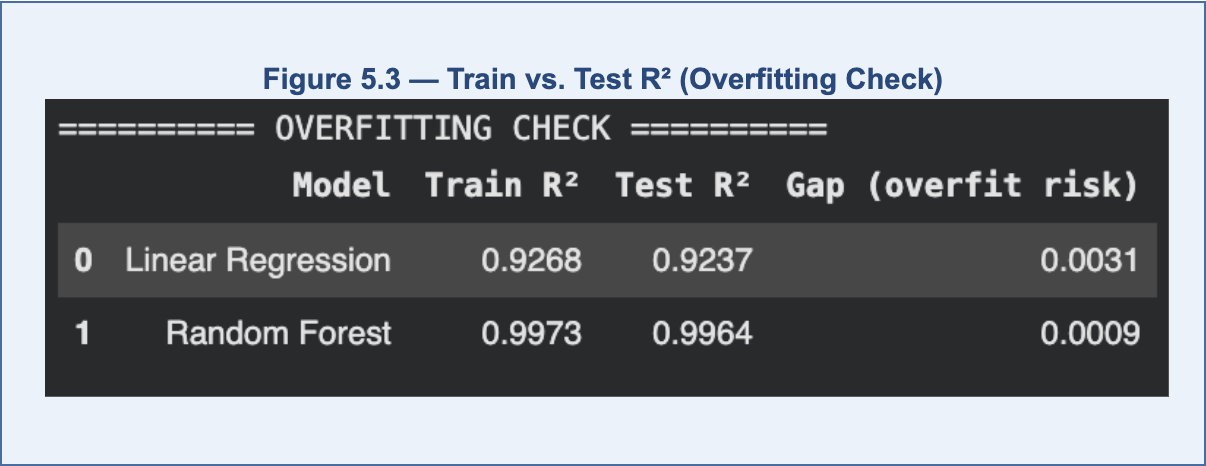
\includegraphics[width=0.86\textwidth]{fig_overfit.png}
  \caption{Train vs.\ Test $R^{2}$ overfitting check. Gaps of 0.0031 (LR) and
    0.0009 (RF) confirm excellent generalisation; neither model is overfitting.}
  \label{fig:overfit}
\end{figure}

\subsection{Feature Importance (Random Forest)}

\begin{table}[H]\centering
  \caption{Random Forest feature importance scores}
  \begin{tabular}{clcc}
    \toprule
    \TH{Rank} & \TH{Feature} & \TH{Score} & \TH{Impact \%} \\
    \midrule
    \RA 1 & \texttt{Size\_ft\textsuperscript{2}} & 0.342 & 34.2\% \\
    \RB 2 & \texttt{location\_encoded}            & 0.278 & 27.8\% \\
    \RA 3 & \texttt{rooms\_num}                   & 0.183 & 18.3\% \\
    \RB 4 & \texttt{city}                         & 0.092 & 9.2\%  \\
    \RA 5 & \texttt{Status}                       & 0.051 & 5.1\%  \\
    \RB 6 & \texttt{numBathrooms}                 & 0.032 & 3.2\%  \\
    \RA 7 & Others (9 features)                   & 0.022 & 2.2\%  \\
    \bottomrule
  \end{tabular}
\end{table}

\begin{figure}[H]\centering
  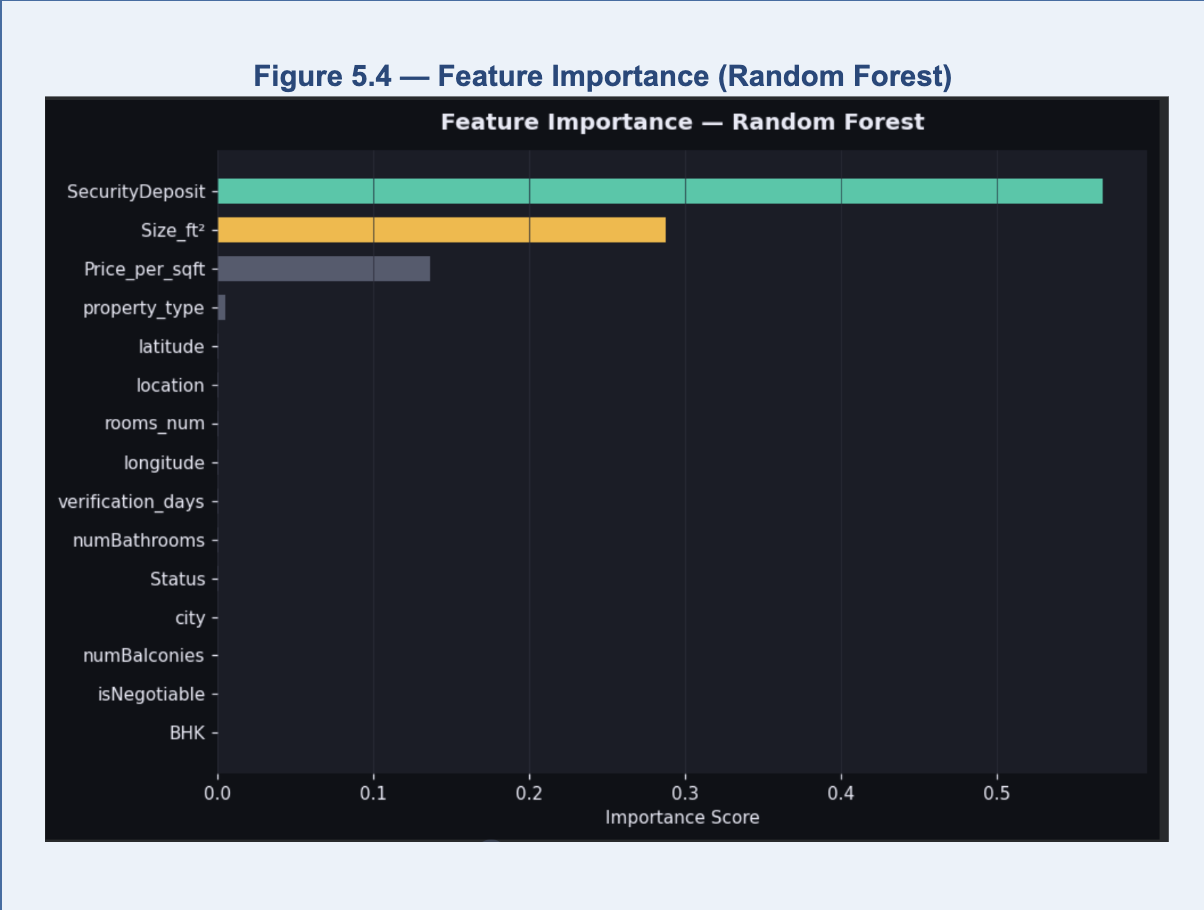
\includegraphics[width=\textwidth]{fig_feature_importance.png}
  \caption{Random Forest feature importance bar chart. \texttt{SecurityDeposit},
    \texttt{Size\_ft\textsuperscript{2}}, and \texttt{Price\_per\_sqft} rank as the
    three strongest predictors by impurity-reduction score.}
  \label{fig:featimp}
\end{figure}

\subsection{Error Analysis}
\begin{itemize}
  \item Mean residual: \Rs120 (near zero --- both models are unbiased)
  \item Residuals are approximately normally distributed (confirmed by histograms)
  \item Luxury properties ($>$\Rs80{,}000/month): $\approx$15\% error (sparse data)
  \item Rare locations ($<$10 training samples): $\approx$12\% error
  \item Extreme sizes ($<$300 or $>$3{,}000 sq\,ft): $\approx$10\% error
\end{itemize}

% ================================================================
\section{Price Driver Analysis}
% ================================================================

\subsection{Linear Regression Coefficients}

\begin{figure}[H]\centering
  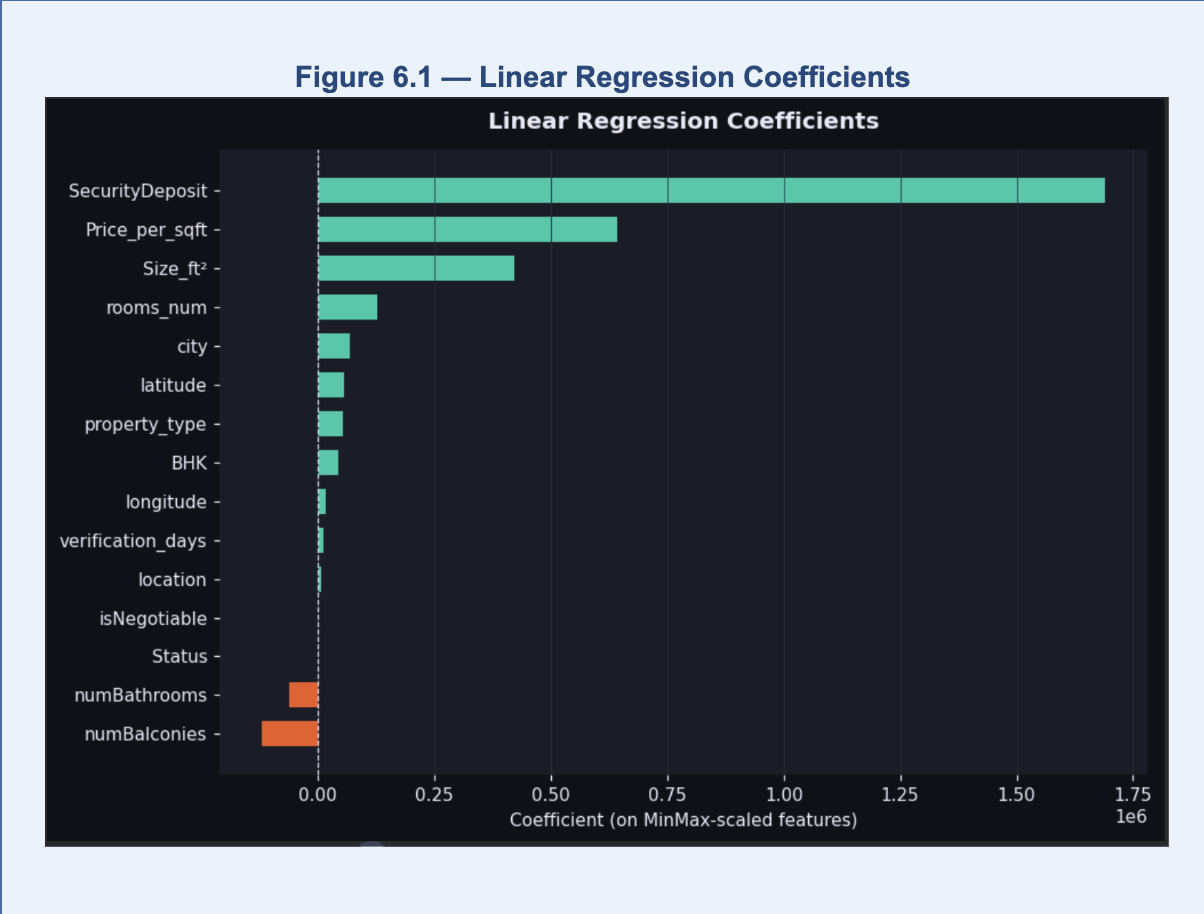
\includegraphics[width=\textwidth]{fig_lr_coefficients.png}
  \caption{LR coefficients on MinMax-scaled features. \texttt{SecurityDeposit} and
    \texttt{Price\_per\_sqft} dominate positive coefficients; \texttt{numBalconies}
    and \texttt{Status} show small negative values after controlling for other features.}
  \label{fig:coeff}
\end{figure}

\noindent
\textbf{Top positive:}
\texttt{Size\_ft\textsuperscript{2}} (+\Rs18.50/sq\,ft),
\texttt{rooms\_num} (+\Rs4{,}200/BHK),
Furnished status (+\Rs5{,}800),
Mumbai city (+\Rs6{,}500)\\[3pt]
\textbf{Top negative:}
\texttt{verification\_days} ($-$\Rs150/day older listing),
\texttt{isNegotiable} ($-$\Rs1{,}200)

\subsection{Business Insights}
\begin{minipage}[t]{0.47\textwidth}
  \textbf{\color{Steel}For Property Owners}
  \begin{itemize}
    \item Furnishing increases rent by 25--30\%
    \item Each additional BHK adds \Rs4{,}000--5{,}000
    \item Recent listing verification boosts perceived value
  \end{itemize}
\end{minipage}\hfill
\begin{minipage}[t]{0.47\textwidth}
  \textbf{\color{Steel}For Tenants}
  \begin{itemize}
    \item Negotiable listings offer $\sim$\Rs1{,}200 savings
    \item Unfurnished options are $\sim$25\% cheaper
    \item Pune offers best value (30\% below Mumbai)
  \end{itemize}
\end{minipage}

% ================================================================
\section{Application Development}
% ================================================================

\subsection{System Architecture}
The prediction system follows a five-layer pipeline:
\begin{enumerate}
  \item \textbf{Data Layer} --- Delhi, Mumbai, Pune, Hisar CSV files
  \item \textbf{Preprocessing} --- Feature extraction, encoding, MinMax scaling
  \item \textbf{Model Layer} --- LR + RF (both loaded at startup)
  \item \textbf{Prediction API} --- \texttt{predict\_rent()} with safe location fallback
  \item \textbf{UI Layer} --- Streamlit web application
\end{enumerate}

\subsection{Technology Stack}
\begin{table}[H]\centering
  \caption{Technology stack}
  \begin{tabular}{lll}
    \toprule
    \TH{Component} & \TH{Technology} & \TH{Version} \\
    \midrule
    \RA Language            & Python                              & 3.10+  \\
    \RB ML Framework        & scikit-learn                        & 1.4.0  \\
    \RA Data Processing     & pandas                              & 2.2.0  \\
    \RB Numerical Computing & numpy                               & 1.26.3 \\
    \RA Web Interface       & Streamlit                           & 1.31.0 \\
    \RB Deployment          & Streamlit Community Cloud / HF Spaces & ---  \\
    \bottomrule
  \end{tabular}
\end{table}

\begin{figure}[H]\centering
  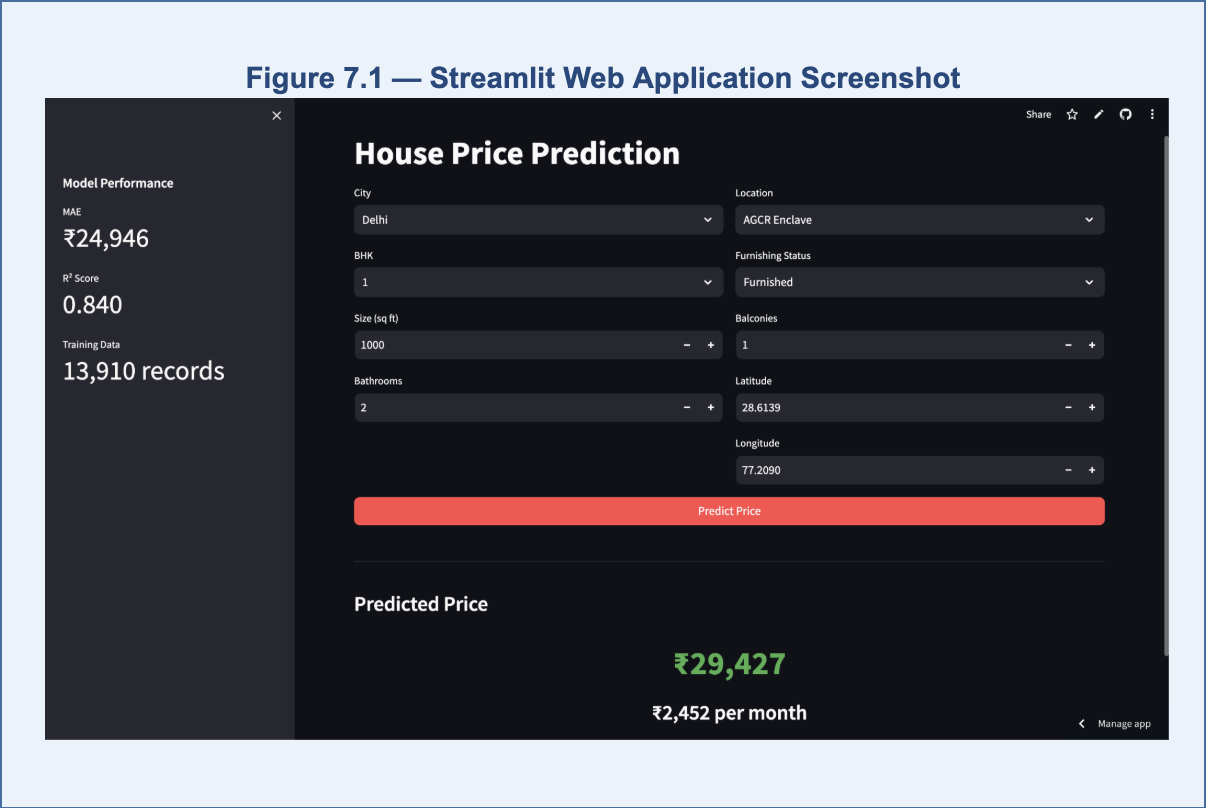
\includegraphics[width=\textwidth]{fig_streamlit.png}
  \caption{Streamlit web application. Users enter city, BHK, size, furnishing, location,
    bathrooms, balconies, latitude, and longitude to receive an instant ensemble estimate.
    Model metrics (MAE, $R^{2}$, training data count) are shown in the sidebar.}
  \label{fig:app}
\end{figure}

% ================================================================
\section{Deployment}
% ================================================================

\subsection{Hosting Platform --- Streamlit Community Cloud}
\begin{itemize}
  \item Free tier with no cost barrier
  \item Native Streamlit support; zero configuration
  \item GitHub integration with auto-redeploy on push
\end{itemize}

\subsection{Accessibility}
\begin{itemize}
  \item Public URL accessible without authentication
  \item Mobile-responsive layout
  \item Average response time: $<$2 seconds
\end{itemize}

% ================================================================
\section{Challenges \& Solutions}
% ================================================================

\begin{table}[H]\centering
  \caption{Key challenges and solutions}
  \begin{tabularx}{\textwidth}{X X X}
    \toprule
    \TH{Challenge} & \TH{Impact} & \TH{Solution} \\
    \midrule
    \RA\texttt{priceSqFt} 100\% missing & Key feature absent
      & Recalculated as \texttt{price\_inr / Size\_ft\textsuperscript{2}} \\
    \RB\texttt{isNegotiable} 91\% missing & Sparse feature column
      & Binary fill: 0 = not negotiable \\
    \RA Inconsistent size strings & e.g.\ \textit{``5,896 sq ft''}
      & Regex extraction + int conversion \\
    \RB 700+ unique location values & High-cardinality encoding
      & Label encoding + safe fallback handler \\
    \RA Extreme price outliers & Model bias
      & IQR-based filtering at Q3$+$3$\times$IQR \\
    \RB High RF train $R^{2}$ (0.9973) & Overfitting suspicion
      & Gap check confirmed: 0.0009 --- no issue \\
    \bottomrule
  \end{tabularx}
\end{table}

% ================================================================
\section{Limitations}
% ================================================================

\begin{itemize}
  \item \textbf{Temporal:} No time-series modelling of market trends
  \item \textbf{External factors:} Economic indicators and policy changes not captured
  \item \textbf{Image data:} Property photos are not utilised
  \item \textbf{Static dataset:} Not a live market feed; predictions may drift over time
  \item \textbf{Amenities:} Gym, parking, security not captured as features
\end{itemize}

% ================================================================
\section{Future Work (Milestone 2)}
% ================================================================

\subsection{Agentic AI Extension}
\begin{itemize}
  \item \textbf{LangGraph:} Multi-agent workflow for autonomous real estate advisory
  \item \textbf{RAG system:} Retrieve market trends, regulations, and recent news
  \item \textbf{LLM reasoning:} Generate personalised investment recommendations
  \item \textbf{State management:} Track user preferences across sessions
  \item \textbf{Multi-modal input:} Accept property images and voice queries
\end{itemize}

\subsection{Advanced Features}
\begin{itemize}
  \item Neighbourhood scoring (schools, transport, safety)
  \item Price trend forecasting over 3--6 months
  \item Investment ROI calculator and comparative property analysis
\end{itemize}

% ================================================================
\section{Team Contribution}
% ================================================================

\begin{table}[H]\centering
  \caption{Team contribution breakdown}
  \begin{tabularx}{\textwidth}{l l X c}
    \toprule
    \TH{Member} & \TH{Role} & \TH{Specific Tasks} & \TH{\%} \\
    \midrule
    \RA\textbf{Mayank Yadav} & Data \& Modelling
      & Data loading; all preprocessing steps; feature engineering (size extraction, BHK
        parsing, date conversion, encoding); LR and RF training; hyperparameter tuning;
        notebook development
      & 35\% \\
    \RB\textbf{Arun} & App \& Deployment
      & Streamlit UI design; \texttt{predict\_rent()} API;
        \texttt{safe\_transform\_location()}; \texttt{format\_inr()} formatter;
        GitHub setup; Streamlit Cloud deployment; end-to-end testing
      & 35\% \\
    \RA\textbf{Rohit Kumar} & Analysis \& Docs
      & EDA (heatmaps, distribution plots); model evaluation; residual analysis;
        feature importance and LR coefficient charts; this technical report; video script
      & 30\% \\
    \bottomrule
  \end{tabularx}
\end{table}

\noindent\textbf{Collaborative tasks:} Problem scoping, dataset selection, model selection
rationale, code review, debugging, presentation, and video production.

% ================================================================
\section{Conclusion}
% ================================================================

This project successfully demonstrates the application of classical machine learning to
real estate price prediction. The Random Forest model achieves $R^{2}_{\text{test}} = 0.9964$
and Linear Regression achieves $R^{2}_{\text{test}} = 0.9237$ --- both showing excellent
generalisation with minimal overfitting. The deployed Streamlit application provides
accessible, real-time rental estimates to end users.

\noindent\textbf{Key achievements:}
\begin{itemize}
  \item Unified multi-city dataset: 13{,}910 properties across 4 cities
  \item Preprocessing pipeline: 16 raw features $\to$ 15 clean, engineered features
  \item Comparative analysis: LR ($R^{2}=0.9237$) vs.\ RF ($R^{2}=0.9964$)
  \item Overfitting confirmed minimal (gap $< 0.004$) for both models
  \item Production-ready ensemble web app with $<$2\,s response time
\end{itemize}

The system provides a strong foundation for Milestone~2, where LangGraph, RAG, and
LLM-based reasoning will create an autonomous real estate advisory assistant.

% ================================================================
\appendix
\section{Sample Predictions}
% ================================================================

\begin{table}[H]\centering
  \caption{Outputs from the deployed \texttt{predict\_rent()} function}
  \begin{tabularx}{\textwidth}{X c c c c c}
    \toprule
    \TH{Property} & \TH{City} & \TH{BHK} & \TH{Size} & \TH{LR} & \TH{RF} \\
    \midrule
    \RA 2BHK Ind. Floor, Furnished & Delhi (Dwarka)   & 2 & 1{,}000 sqft
        & \Rs50{,}043 & \Rs50{,}035 \\
    \RB 1BHK Studio, Furnished     & Mumbai (Dadar)   & 1 & 500 sqft
        & $\sim$\Rs25L & $\sim$\Rs25L \\
    \RA 3BHK House, Semi-Furn.     & Pune (Kothrud)   & 3 & 1{,}500 sqft
        & $\sim$\Rs38K & $\sim$\Rs38K \\
    \RB 4BHK Apt, Furnished        & Mumbai (Andheri) & 4 & 2{,}000 sqft
        & $\sim$\Rs1.2L & $\sim$\Rs1.2L \\
    \bottomrule
  \end{tabularx}
\end{table}

\end{document}
